\documentclass[8pt]{article}
%%%%%%%%%%%%%%%%%%%%%%%%%%%
% Packages
%%%%%%%%%%%%%%%%%%%%%%%%%%%
\usepackage{hyperref}
\hypersetup{
  pdfauthor={Marco Arieli Herrera-Valdez},
  pdftitle={}
  pdftex,
  colorlinks=true,
  urlcolor=Bittersweet,
  linkcolor=blue,
  pdftoolbar=true,
  pdfmenubar=true,
  citecolor=Purple,
  filecolor=blue,
}
%\usepackage[spanish,es-nodecimaldot]{babel}
\usepackage{lscape}
\usepackage{setspace}
%\setstretch{1.1}
%\doublespacing
\usepackage[utf8]{inputenc}
%\usepackage[latin1]{inputenc}
%\usepackage[applemac]{inputenc}
%% Only if the base font of the document is to be different, say sans serif
% Text layout
\usepackage[T1]{fontenc}
\usepackage[scaled=0.92]{helvet}
\renewcommand*\familydefault{\sfdefault}
\usepackage{authblk}
\usepackage{graphicx}
\usepackage{python}
\usepackage{mathtools,amsfonts,amssymb,amsmath}
\usepackage[dvipsnames,svgnames,hyperref,table]{xcolor}
%\usepackage{xcolor}
\usepackage{microtype}
\usepackage{sidecap}
%\hypersetup{pdfpagemode=FullScreen}
%\usepackage[left=2.5cm,right=2.5cm,top=0cm,bottom=2cm,includehead]{geometry}
\usepackage{geometry}
\usepackage{fancyhdr}
%\pagestyle{fancyplain}
%\pagestyle{plain}
% The color packages must appear before the pdfpages package
%\usepackage{chemarr}
\usepackage{listings}
%\usepackage[normalem]{ulem}
%\usepackage[usenames,svgnames,dvipsnames]{xcolor}
%\usepackage[dvipsnames,svgnames,usenames]{xcolor}
%\usepackage{booktabs} % Top and bottom rules for table
\usepackage[font=small,labelfont=bf]{caption}
\usepackage{wrapfig}
%\usepackage{subfigure}
%\usepackage{beamerthemesplit}
\usepackage{boldline}
\usepackage{multirow}
\usepackage{multicol}
\usepackage{longtable}
\usepackage{times}
\usepackage{animate}
\usepackage{pdfpages}
\usepackage{url}
%\usepackage{multimedia}
%\usepackage{movie15}
%\usepackage{media9}
\usepackage{verbatim}
%\usepackage{pgflibraryarrows}
%\usepackage{pgflibraryshapes}
\usepackage{tikz}
%\usetikzlibrary{arrows,shapes,matrix,chains,calc,positioning}
%\usetikzlibrary{trees,mindmap}
\usepackage{ifthen}
\usepackage{animate}

% To get the envelope in the author list
\usepackage[misc]{ifsym}
%\usepackage[misc,geometry]{ifsym}

%\Letter after the name of the corresponding author

% --------------------------------------
% Bibliography
% --------------------------------------
%\usepackage[sort&compress]{natbib}
\usepackage[round,sort&compress]{natbib}
%\usepackage[numbers,sort&compress]{natbib}
%\bibliographystyle{plainnat}

% ------------------------------------------------
% Abbreviations and other commands
% ------------------------------------------------
\newcommand{\lrRound}[1]{\left(#1\right)}
\newcommand{\lrSquare}[1]{\left[#1\right]}
\newcommand{\lrSet}[1]{\left\{#1\right\}}
\newcommand{\lrAbs}[1]{\left|#1\right|}
\newcommand{\lrNorm}[1]{\left\|#1\right\|}
\newcommand{\prob}[1]{\mathbf{P}\left\{ #1\right\}}
\newcommand{\eg}{\textit{e.g.}}
\newcommand{\ie}{\textit{i.e.}}
\newcommand{\potassium}{{K$^+$}}
\newcommand{\kalium}{{K$^+$}}
\newcommand{\hydrogen}{{H$^+$}}
\newcommand{\sodium}{{Na$^+$}}
\newcommand{\natrium}{{Na$^+$}}
\newcommand{\calcium}{{Ca$^{2+}$}}
\newcommand{\chloride}{{Cl$^{-}$}}
\newcommand{\magnessium}{{Mg$^{2+}$}}
\newcommand{\concRatio}[1]{ \frac{ [{#1}]_{0} }{ [{#1}]_{1}} } 
\newcommand{\extConc}[1]{[#1]_{0}}
\newcommand{\intConc}[1]{[#1]_{1}}
\newcommand{\concNa}{[Na]}
\newcommand{\concCa}{[Ca]}
\newcommand{\concCl}{[Cl]}
\newcommand{\concK}{[K]}
\newcommand{\felis}{{{$I_{cyc}$}}}
\newcommand{\icyc}{{{$I_{cyc}$}}}
\newcommand{\Avogadro}{N_{\mathrm{A}}}
\newcommand{\absTemp}{\mathrm{T}}
\newcommand{\GasConstant}{\mathrm{R}}
\newcommand{\Faraday}{\mathrm{F}}
\newcommand{\hPlanck}{\mathrm{h}}
\newcommand{\kBoltzmann}{\mathrm{k}}
\newcommand{\kT}{\mathrm{kT}}
\newcommand{\qElementary}{\mathrm{q}}
\newcommand{\hqovertwokT}[1]{\frac{\mathrm{e_0}#1}{2\mathrm{kT}}}
\newcommand{\hqoverkT}[1]{\frac{\bathroom{e_0}#1}{\mathrm{kT}}}
\def\qovertwokT{\mathrm{\frac{e_0}{2kT}}}
\def\qoverkT{\mathrm{\frac{e_0}{kT}}}
\newcommand{\trace}[1]{{\mathrm{Tr}(#1)}}
\newcommand{\tSm}{{\mathrm{Sm}}}
\newcommand{\tSy}{{\mathrm{Sy}}}
\newcommand{\tSt}{{\mathrm{St}}}
\newcommand{\tF}{{\mathrm{F}}}
\newcommand{\tLFP}{{\mathrm{LFP}}}
\newcommand{\tATP}{{\mathrm{ATP}}}
\newcommand{\tADP}{{\mathrm{ADP}}}
\newcommand{\tCaATP}{{\mathrm{CaATP}}}
\newcommand{\tP}{{\mathrm{P}}}
\newcommand{\tNa}{{\mathrm{Na}}}
\newcommand{\tNaK}{{\mathrm{NaK}}}
\newcommand{\tNaKa}{{\mathrm{NaKa}}}
\newcommand{\tNaP}{{\mathrm{NaP}}}
\newcommand{\tNaT}{{\mathrm{NaT}}}
\newcommand{\tNaH}{{\mathrm{NaH}}}
\newcommand{\tNaCa}{{\mathrm{NaCa}}}
\newcommand{\tNaKCl}{{\mathrm{NaKCl}}}
\newcommand{\tKCl}{{\mathrm{KCl}}}
\newcommand{\tCa}{{\mathrm{Ca}}}
\newcommand{\tCl}{{\mathrm{Cl}}}
\newcommand{\tCaL}{{\mathrm{CaL}}}
\newcommand{\tE}{{\mathrm{E}}}
\newcommand{\tExtra}{{\mathrm{Extra}}}
\newcommand{\tExt}{{\mathrm{Ext}}}
\newcommand{\tI}{{\mathrm{I}}}
\newcommand{\tGlu}{{\mathrm{GluA}}}
\newcommand{\tAMPA}{{\mathrm{AMPA}}}
\newcommand{\tGABA}{{\mathrm{GABA}}}
\newcommand{\tGabaA}{{\mathrm{GabaA}}}
\newcommand{\tACh}{{\mathrm{ACh}}}
\newcommand{\tS}{{\mathrm{S}}}
\newcommand{\tSK}{{\mathrm{SK}}}
\newcommand{\tH}{{\mathrm{H}}}
\newcommand{\tK}{{\mathrm{K}}}
\newcommand{\tKaD}{{\mathrm{KaD}}}
\newcommand{\tKD}{{\mathrm{KD}}}
\newcommand{\tL}{{\mathrm{L}}}
\newcommand{\INa}{{I_\mathrm{Na}}}
\newcommand{\INaT}{{I_\mathrm{NaT}}}
\newcommand{\ICa}{{I_{\mathrm{Ca}}}}
\newcommand{\ICaL}{{I_{\mathrm{CaL}}}}
\newcommand{\IKD}{{I_{\mathrm{KD}}}}
\newcommand{\IKaD}{{I_{\mathrm{KaD}}}}
\newcommand{\IK}{{I_{\mathrm{K}}}}
\newcommand{\IAMPA}{{I_{\mathrm{AMPA}}}}
\newcommand{\INMDA}{{I_{\mathrm{NMDA}}}}
\newcommand{\IGABA}{{I_{\mathrm{GABA}}}}
\newcommand{\INaKATP}{{I_{\mathrm{NaK}}}}
\newcommand{\INaK}{{I_{\mathrm{NaK}}}}
\newcommand{\INaKa}{{I_{\mathrm{NaKa}}}}	
\newcommand{\INaCaX}{{I_{\mathrm{NaCa}}}}
\newcommand{\ILeak}{{I_{\mathrm{L}}}}
\newcommand{\stimtop}{{\textit{Top}}}
\newcommand{\stimup}{{\textit{Up}}}
\newcommand{\stimdown}{{\textit{Down}}}
\newcommand{\diffop}[2]{{\partial_{#1} #2}}
%
\newcommand{\splitPage}[4]{
\begin{minipage}{#1\textwidth}
{#2}
\end{minipage}%
\begin{minipage}{#3\textwidth}
{#4}
\end{minipage}
}

\newcommand{\figref}[1]{{Fig.~\ref{#1}}}
\newcommand{\figtworefs}[2]{{Figs.~\ref{#1}~and~\ref{#2}}}
\newcommand{\figrefs}[2]{{Figs.~\ref{#1}-\ref{#2}}}
\newcommand{\req}[1]{{Eq.~\eqref{#1}}}
\newcommand{\rtwoeqs}[2]{{Eqs.~\eqref{#1}~and~\eqref{#2}}}
\newcommand{\reqs}[2]{{Eqs.~\eqref{#1}-\eqref{#2}}}
\newcommand{\eqn}[1]{\begin{equation}#1\end{equation}}
\newcommand{\eqna}[1]{\begin{eqnarray}#1\end{eqnarray}}
\newcommand{\smalleq}[1]
{\begin{equation}{\small #1}\end{equation}}
\newcommand{\smalleqna}[1]{ 
  \begin{small} 
    \begin{eqnarray} #1 \end{eqnarray} 
  \end{small}
}
\newcommand{\tinyeqna}[1]{ 
  \begin{tiny} 
    \begin{eqnarray} #1 \end{eqnarray} 
  \end{tiny}
}
% LaTeX beamer
\newcommand{\slide}[1]{\begin{frame}#1\end{frame}}
\newcommand{\from}[1]{{\tiny From #1.}}
\newcommand{\fuente}[1]{{\tiny #1}}
\newcommand{\source}[1]{{\tiny #1}}
\newcommand{\sS}[3]{{{#1}_{#2}^{#3}}}

\newcommand{\email}{\textrm{\Letter}}
\newcommand{\corrAuthor}{\textrm{\Letter}}
\newcommand{\insp}{{National Institute of Public Health}}
\newcommand{\cisei}{{Center for Research on Infectious Diseases}}
\newcommand{\imate}{{Mathematics Institute}}
\newcommand{\unam}{{National Autonomous University of Mexico}}
\newcommand{\ua}{{University of  Arizona}}
\newcommand{\uprc}{{University of Puerto Rico in Cayey}}
\newcommand{\mbi}{{Mathematical Biosciences Institute}}
\newcommand{\osu}{{Ohio State University}}
\newcommand{\asu}{{Arizona State University}}
\newcommand{\sols}{{School of Life Sciences}}
\newcommand{\smss}{{School of Mathematical Sciences and Statistics}}
\newcommand{\mcmsc}{{Mathematical, Computational, and Modelling Sciences Center}}
\newcommand{\shesc}{School of Human Evolution and Social Change}
%
 \newcommand{\INSP}{{Instituto Nacional de Salud Pública}}
\newcommand{\CISEI}{{Centro de Investigación Sobre Enfermedades Infecciosas}}
\newcommand{\UNAM}{{Universidad Nacional Aut\'onoma de M\'exico}}
\newcommand{\IM}{{Instituto de Matem\'aticas}}
\newcommand{\IF}{{Instituto de F\'isica}}
\newcommand{\FC}{{Facultad de Ciencias}}
\newcommand{\DM}{{Departamento de Matem\'aticas}}
% \newcommand{\ua}{{Universidad de  Arizona}}
% \newcommand{\asu}{{Universidad Estatal de Arizona}}
% \newcommand{\uprc}{{Universidad de Puerto Rico en Cayey}}
% \newcommand{\mbi}{{Instituto de Biociencias Matem\UTF{00C3}\UTF{00A1}ticas}}
% \newcommand{\osu}{{Universidad Estatal de Ohio}}
% ------------------------------------------------

%%%%%%%%%%%%%%%%%%%%%%%%%%%
% Edits and reviews
%%%%%%%%%%%%%%%%%%%%%%%%%%%
\newcommand{\aquimequede}{
\vspace{1cm} \textcolor{red}
{\textbf{AQUI ME QUEDE}} \\
\vspace{1cm}}
\newcommand{\mahv}[1]{\textcolor{gray}{$^{MAHV:}$}\textcolor{orange}{#1} }




%%%%%%%%%%%%%%%%%%%%%%%%%%%
% Colored sections
%%%%%%%%%%%%%%%%%%%%%%%%%%%
\newcommand{\headcolor}[1]{\textcolor{Bittersweet}{#1}}
\newcommand{\colorsection}[1]{\section*{\headcolor{#1}}}
\newcommand{\colorsubsection}[1]{\subsection*{\headcolor{#1}}}
\newcommand{\colorparagraph}[1]{\paragraph{\headcolor{#1}}}
\definecolor{lightGray}{rgb}{0.92,0.92,0.92}


%%%%%%%%%%%%%%%%%%%%%%%%%%%
% Figure settings and inclusion/exclusion of figures from the compilation
%%%%%%%%%%%%%%%%%%%%%%%%%%%

\newcommand{\figu}[3]{
\begin{figure}{\begin{center}#3\end{center}}\caption{#1}\label{#2}\end{figure}}
\newcommand{\tablFigu}[3]{
\begin{table}\caption{#1}\label{#2}\begin{center}{#3}\end{center}\end{table}}
%
\newcommand{\smallcaption}[1]{\begin{small}\caption{{#1}}\end{small}}
%\renewcommand{\caption}[1]{\caption{\begin{small}#1\end{small}}}
\usepackage{comment}
%\excludecomment{cond}
\includecomment{cond}
\newcommand{\showfigs}[1]{}
\begin{cond}
\renewcommand{\showfigs}[1]{\begin{center}#1\end{center}}
\end{cond}

% --------------------------------------
% mahvMacros
% --------------------------------------
% For supplements
% --------------------------------------
%\newcommand{\hbAppendixPrefix}{A}
%
%\renewcommand{\thefigure}{\hbAppendixPrefix\arabic{figure}}
%\setcounter{figure}{0}
%\renewcommand{\thetable}{\hbAppendixPrefix\arabic{table}} 
%\setcounter{table}{0}
%\renewcommand{\theequation}{\hbAppendixPrefix\arabic{equation}} 
%\setcounter{equation}{0}


\newenvironment{suppFig}[4]{
  \begin{figure}[h]
    \begin{center}
      {\includegraphics[#4]{#3}} \caption{\small #1} \label{#2}
    \end{center}
  \end{figure}}

\newenvironment{tab}[3]{
\begin{table}
\begin{center}
{#3} \caption{\small #1} \label{#2}
\end{center}
\end{table}}

% Operators
\DeclareMathOperator{\Tr}{Tr}
\newcommand{\re}[1]{ {\mathfrak{Re}} \left( {#1} \right)}
\newcommand{\im}[1]{ {\mathfrak{Im}} \left( {#1} \right)}
% Transpose upperscript
\newcommand{\transp}[1]{#1^{\mathsmaller T}}

% Column vectors. Usage:
% \colvector{a\\b\\c\\d\\e}
\newcommand{\colvector}[1]{\begin{pmatrix}#1\end{pmatrix}} 

% Column vectors. Usage:
% \colvec{5}{a}{b}{c}{d}{e}
\newcount\colveccount
\newcommand*\colvec[1]{
        \global\colveccount#1
        \begin{pmatrix}
        \colvecnext
}
\def\colvecnext#1{
        #1
        \global\advance\colveccount-1
        \ifnum\colveccount>0
                \\
                \expandafter\colvecnext
        \else
                \end{pmatrix}
        \fi
}

% ----------------------------------
% Code listing 
% ----------------------------------
%\lstdefinestyle{customPython}{
%  language=Python,
%  belowcaptionskip=1\baselineskip,
%  breaklines=true,
%  %frame=L,
%  xleftmargin=\parindent,
%  showstringspaces=false,
%  basicstyle=\footnotesize\ttfamily,
%  keywordstyle=\bfseries\color{green!40!black},
%  commentstyle=\itshape\color{purple!40!black},
%  identifierstyle=\color{blue},
%  stringstyle=\color{orange},
%}

%\newcommand<>{\hover}[1]{\uncover#2{%
% \begin{tikzpicture}[remember picture,overlay]%
% \draw[fill,opacity=0.4] (current page.south west)
% rectangle (current page.north east);
% \node at (current page.center) {#1};
% \end{tikzpicture}}
%}

\usepackage[utf8]{inputenc}
\usepackage[position=top]{subfig}
\usepackage{tkz-berge}
\usetikzlibrary{arrows,petri,topaths}
\tikzstyle{vertex}=[circle, draw, inner sep=3pt, minimum size=5pt]
\newcommand{\vertex}{\node[vertex]}
\setstretch{1.3}
%
\title{Dinámica inicial de la epidemia de Covid-19 en en mundo y en México }
\author{Marco Arieli Herrera-Valdez}
\date{April 2020}
%
\begin{document}
%
%\begin{flushleft}
%\begin{Large}
%{Estimaciones y análisis de la dinámica inicial de la mortalidad de casos epidemia de Covid-19 en México a partir de los datos mundiales}
%\end{Large}\\
%\smallskip
%\begin{large}
%Carlos Ignacio Herrera-Nolasco$^1$, Eugenia O'Reilly-Regueiro$^{4,\email}$,
%Marco Arieli Herrera-Valdez$^{1,\email}$
%\end{large}\\
%\smallskip
%$^1$ Departamento de Matemáticas, Facultad de Ciencias, Universidad Nacional Autónoma de México\\
%$^4$ Instituto de Matemáticas, Facultad de Ciencias, Universidad Nacional Autónoma de México\\
%$\email$ marcoh@ciencias.unam.mx, eugenia@im.unam.mx
%\end{flushleft}
%
% ---------------------------------------------------------
\section*{Análisis de las primeras semanas de la dinámica de la pandemia de {Covid-19} y estudio de mecanismos macroscópicos de propagación con apoyo de modelos estocásticos}
Carlos Ignacio Herrera-Nolasco, Eugenia O'Reilly-Regueiro, Sergio Iván López Ortega, Marco Arieli Herrera-Valdez.


% !TEX root = tsam_Covid19_Mexico.tex
\subsection*{Inferencia de características del curso temporal de Covid-19 a partir de medidas macroscópicas de reportes de casos, recuperaciones y muertes}

\paragraph{Participantes.} Carlos Ignacio Herrera-Nolasco, Eugenia O'Reilly-Regueiro, Sergio Iván López Ortega, Marco Arieli Herrera-Valdez. Este trabajo es parte de un reporte técnico que está siendo editado para su revisión por pares. Se pueden encontrar más detalles y referencias en \url{https://scab-unam.github.io/tsam_Covid-19/tsam_Covid19_analysis/tsam_Covid19_cfrAnalysis_ReadMe.html}
\paragraph{Retrasos entre comienzo de síntomas y recuperación o muerte a partir de los primeros reportes de caso en el mundo}


?`Es posible observar en los reportes de casos hechos a nivel mundial indicaciones del tiempo que tarda una persona en morir por complicaciones de Covid-19 a partir comienza a tener síntomas? Es decir, ?`es posible estimar el retraso en entre la muerte y la manifestación de síntomas desde una perspectiva macroscópica de los casos y los decesos por caso en distintos países?


%
\begin{figure}[h]
\begin{minipage}{0.5\textwidth}
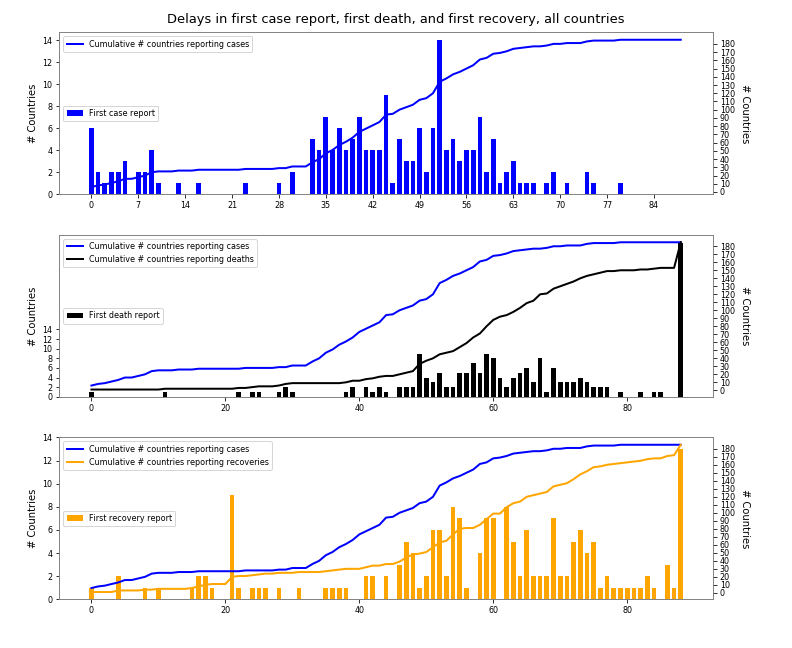
\includegraphics[width=\textwidth]{../tsam_Covid19_analysis/figures/tsam_Covid19_JHU_reportArrivals_AllCountries}
\end{minipage}%
\begin{minipage}{0.5\textwidth}
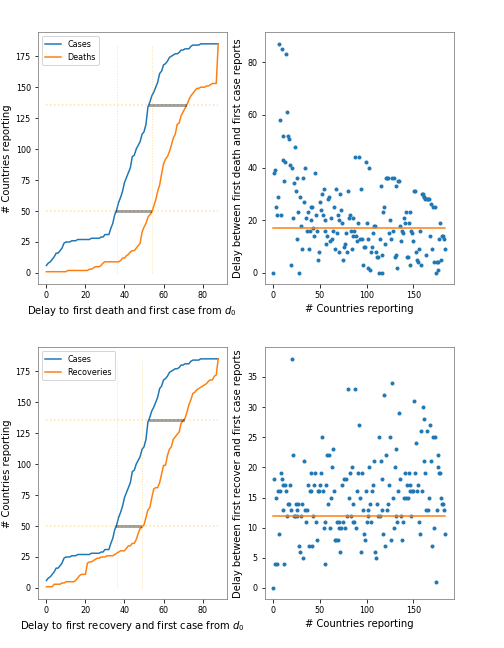
\includegraphics[width=\textwidth]
{../tsam_Covid19_analysis/figures/tsam_Covid19_JHU_delays_caseDeaths}
\end{minipage}%
\caption{Retrasos entre reportes de casos (arriba), muertes (en medio), y recuperaciones (abajo). }. \label{fig:reportArrivals}
\end{figure}


La respuesta está en analizar el retraso entre primer reporte de casos y el primer reporte de muertes en distintos países. La mayoría de los países que primero reportaron casos también reportó muertes (sin retraso). Sin embargo, a medida que pasaron las semanas, se fue observando una tendencia que arroja un retraso promedio de 18 días entre primer caso confirmado y primera muerte en varios países (\figref{fig:reportArrivals}). Es posible medir dicha diferencia utilizando distintos métodos, entre los cuales está simplemente medir la distancia horizontal entre las gráficas acumuladas del número de países que han reportado primer caso o muerte, respectivamente (\figref{fig:reportArrivals}, en medio izquierda, y arriba a la derecha). 
De esa forma también es posible medir el retraso entre reportes de casos y primera recuperación, que resulta ser de aproximadamente 12 días  (\figref{fig:reportArrivals} paneles de abajo).

\bigskip
\paragraph{Contribución de grupos de riesgo por edad a la dinámica de fallecimientos por caso.}
La fatalidad en casos confirmados depende de factores que incluyen la calidad de los servicios de salud, y el acceso a dichos servicios, entre otros. 
Sin embargo, es posible observar algunas similitudes macroscópicas en el comportamiento de las defunciones por Covid-19 en lugares que podría pensarse que los fallecimientos presentarían comportamientos muy distintos , como China y Korea del Sur por un lado, o lugares como Italia, por el otro. 
En Korea del Sur y China, el control es muy estricto y la cuantificación de casos ha sido masiva. 
En cambio en Italia, donde la estructura poblacional es distinta, ha habido más fallecimientos por Covid-19, y ha sido rebasado el sistema de salud al grado de tener que negar el uso de respiradores a la gente. 
Sin embargo, en los tres paises el cociente de fatalidad de casos (CFR por sus siglas en inglés) tiene muchas similitudes (\figref{fig:estimates}, izquierda arriba), que se pueden explotar para obtener las contribuciones relativas de los fallecimientos por Covid-19 (\figref{fig:estimates}, izquierda abajo) por cada grupo de edad al total de muertes observadas, y usar esas estimaciones. 

Por su similitud, es posible usar los pesos relativos de las defunciones de los distintos grupos de edad y  hacer distintas predicciones para el caso de México (\figref{fig:estimates}).


\begin{figure}[h]
\centering
\begin{minipage}{0.5\textwidth}
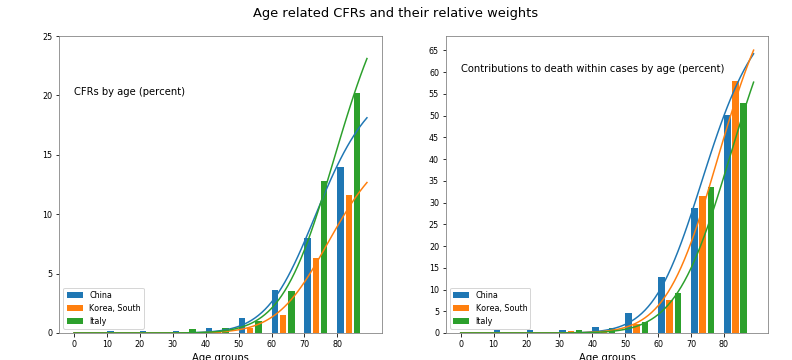
\includegraphics[width=0.9\textwidth]{../tsam_Covid19_analysis/figures/tsam_Covid19_JHU_cfr+propDeathCases_ByAge_China+SKorea+Italy_OneFigure.png}
\end{minipage}%
\begin{minipage}{0.5\textwidth}
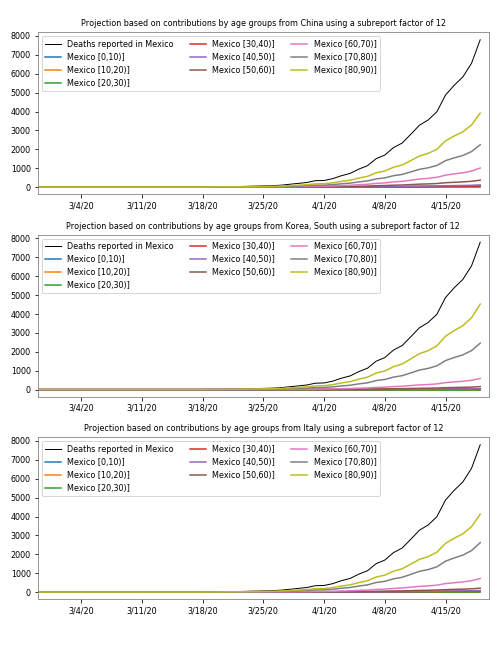
\includegraphics[width=0.9\textwidth] {../tsam_Covid19_analysis/figures/tsam_Covid19_JHU_cfr+propDeathCasesByAgeTS_EstimatesMexico_subReportFactor12.png}
\end{minipage}
\caption{(Izquierda) Contribuciones de distintos grupos de edad a la fatalidad por casos en China, Korea del Sur, e Italia. (Derecha) Estimaciones de fatalidad para México tomando en cuenta grupos de edad, con los datos de China, Korea del Sur, e Italia, calculado hasta el 11 de abril de 2020, y usando un factor de ajuste por subreporte igual a 12. }\label{fig:estimates}
\end{figure}

Las proyecciones obtenidas usando los datos de los distintos países son similares. Hay que tomar en cuenta que estos datos no han sido ajustados con respecto a subreporte. Por ejemplo, ajustando los datos con un factor de 12 por subreporte, la estimación de  muertes de adultos de más de 70 años para México es  de alrededor 4000 para el 19 de abril de 2020. 


Es importante mencionar que estas estimaciones no toman en cuenta la estructura poblacional en México, o la de los países tomados para el análisis, pero esa información está normalizada en el cálculo de los cocientes de fatalidad por caso (\figref{fig:estimates}). 







% !TEX root = ../tsam_Covid19_Mexico/tsam_Covid19_Mexico.tex



\subsection*{Estimación de fecha de inicio y pico de la epidemia de Covid-19}
\paragraph{Participantes.} Carlos Ignacio Herrera-Nolasco, Marco Arieli Herrera-Valdez. Este trabajo es parte de un reporte técnico que está siendo editado para su revisión por pares. Se pueden encontrar más detalles y referencias en \url{https://scab-unam.github.io/tsam_Covid-19/tsam_Covid19_models/figures/Covid19_Mexico_InitialFit_Herrera-Valdez+Herrera-Nolasco_2020.png}.  

Los casos de Covid-19 se pueden dividir en distintos grupos dependiendo de la duración del periodo de carga viral, que a su vez indica su contribución potencial a la cadena de transmisión. Se puede entonces usar un modelo parecido en esencia al SIR. Sin embargo, hay que distinguir que los recuperados pueden permanecer contagiosos. Es decir, los recuperados pueden seguir participando en la cadena de infección. Para no generar confusiones en ese sentido, dividimos a la población en tres grupos de tamaños $N$, $I$, y $W$ que representan respectivamente los no infectados, infectados, y retirados de la cadena de infección \citep{Herrera}. 
\begin{eqnarray}
N(t+h) &=& N(t) - X_{NA}(t)
\\
I(t+h) &=& X_{NA}(t) + \sum{Y_{Ik}(t): k \in \lrSet{A,M,S,C}}  - D(t)
\\
W(t+h) &=& \sum_{k \in \lrSet{A,M,S,C}} Y_{Ik}(t) 
\end{eqnarray}

\begin{figure}[h] 
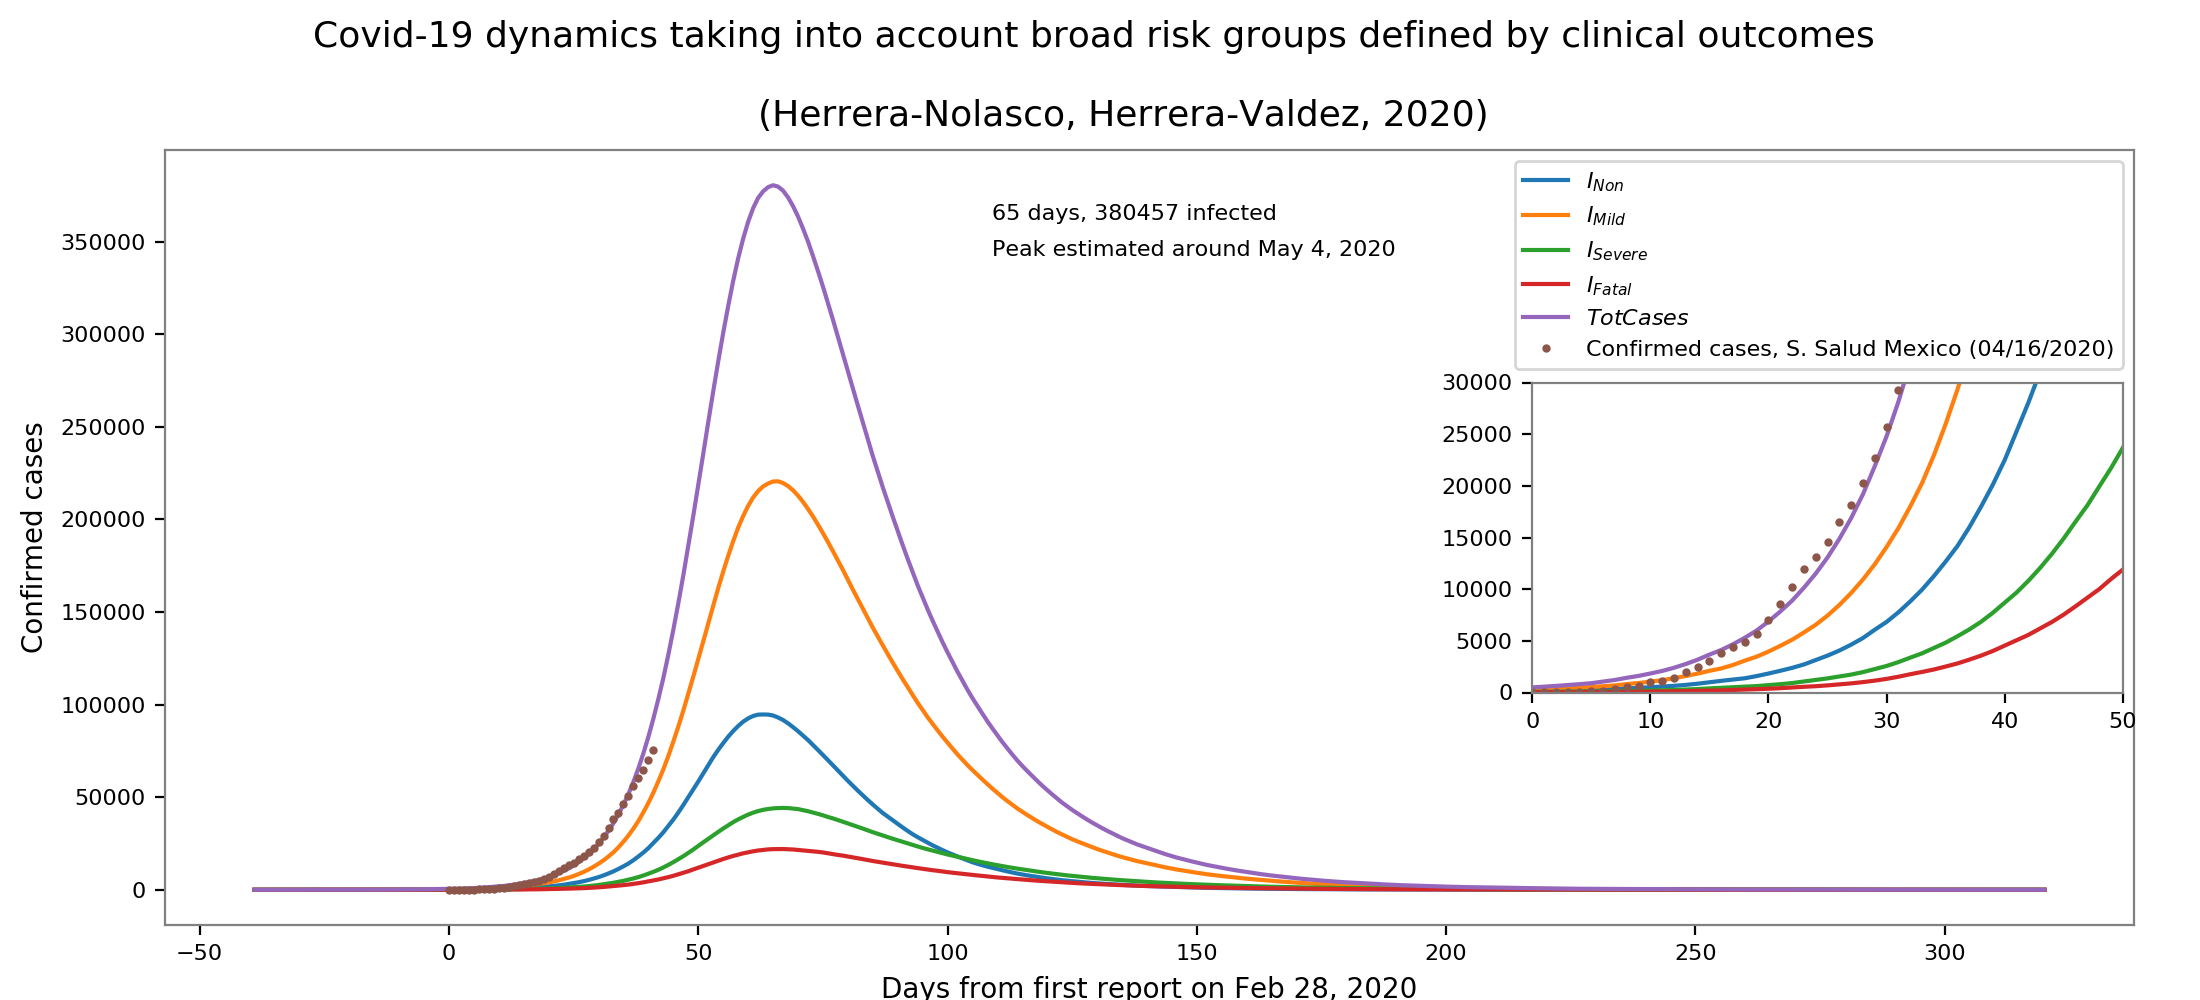
\includegraphics[width=\textwidth]{../tsam_Covid19_models/figures/Covid19_Mexico_InitialFit_Herrera-Valdez+Herrera-Nolasco_2020}
\caption{Estimación de la fecha de inicio y pico de la epidemia ajustando los datos iniciales de la epidemia de Covid-19 en México. La fecha cero representa el 27 de febrero de 2020. La fecha de inicio de la epidemia es aproximadamente 39 días antes, aproximadamente el 20 de enero de 2020.} \label{fig:inicioPicoNIW}
\end{figure}


Los valores esperados de los muestreos del modelo estocástico se pueden utilizar para derivar una ecuación determinista para el régimen en el que los tamaños poblacionales son grandes (Fig.~\ref{}). 
\begin{figure}[h]
\centering
\begin{minipage}{0.65\textwidth}
\begin{eqnarray*}
\partial_{t} x &=& -  \lambda x\\
\partial_{t} y &=& \lambda x - \vec{\gamma} \cdot \vec{y}  - \frac{y_{C}}{\tau_{F}}
\\
\partial_{t} w &=&\vec{\gamma} \cdot \vec{y}
\end{eqnarray*}
\end{minipage}%
\begin{minipage}{0.35\textwidth}
\centering
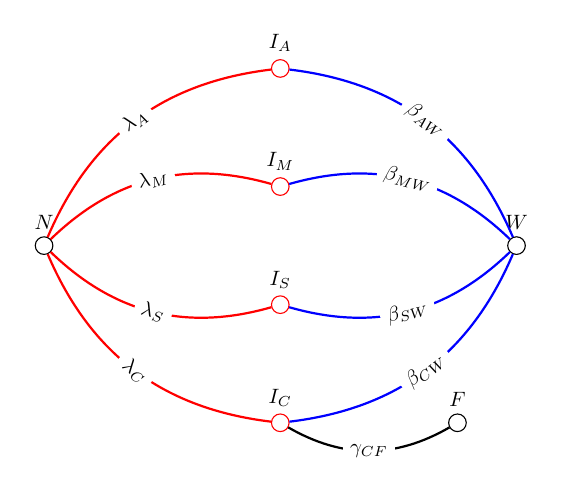
\begin{tikzpicture}[scale=0.75,transform shape]
	\vertex[label=\textcolor{black}{$N$},color=black](N) at (-4,0) { };
	\vertex[label=\textcolor{black}{$I_{A}$},color=red](A) at (0,3) {};
	\vertex[label=\textcolor{black}{$I_{M}$},color=red](M) at (0,1) {};
	\vertex[label=\textcolor{black}{$I_{S}$},color=red](S) at (0,-1) {};
	\vertex[label=\textcolor{black}{$I_{C}$},color=red](C) at (0,-3) {};
	\vertex[label=\textcolor{black}{$W$},color=black](W) at (4,0) { };
	\vertex[label=\textcolor{black}{$F$}](F) at (3,-3) {};
  \tikzstyle{LabelStyle}=[fill=white,sloped]
  \tikzstyle{EdgeStyle}=[bend left]
  \Edge[label=$\lambda_{A}$,color=red](N)(A)
  \Edge[label=$\lambda_{M}$,color=red](N)(M)
  \Edge[label=$\beta_{AW}$,color=blue](A)(W)
  \Edge[label=$\beta_{MW}$,color=blue](M)(W)
  \tikzstyle{EdgeStyle}=[bend right]
  \Edge[label=$\lambda_{S}$,color=red](N)(S)
  \Edge[label=$\lambda_{C}$,color=red](N)(C)
  \Edge[label=$\beta_{SW}$,color=blue](S)(W)
  \Edge[label=$\beta_{CW}$,color=blue](C)(W)
  \Edge[label=$\gamma_{CF}$](C)(F)
\end{tikzpicture}
\end{minipage}%
\caption{Límite determinista del modelo estocástico usado en la \figref{fig:inicioPicoNIW} para simular escenarios de la epidemia de Covid-19 en México. }
\end{figure}


\subsubsection*{Trabajo en progreso.} Continuamos desarrollando modelos estocásticos de dinámica de propagación basados en estimaciones cualitativas similares a las descritas arriba, con la intención de explicar mecanismos subyacentes a la propagación de la epidemia.  
% ---------------------------------------------------------

%\paragraph{Acknowledgments:}


\bibliographystyle{plainnat}
\bibliography{Covid19,epidemiology}
\end{document}
